\documentclass[12pt]{article}
\usepackage{lingmacros}
\usepackage{tree-dvips}
\usepackage{amsmath}
\usepackage{amssymb}
\usepackage{mathpazo}
\usepackage[ngerman]{babel}
\usepackage{fontspec}
\usepackage{algpseudocode}
\usepackage{algorithm}
\usepackage{mathrsfs}
\usepackage{dsfont}
\usepackage{graphicx}
\usepackage{ wasysym }
\usepackage{listings}
\usepackage{ amssymb }
\usepackage[hypcap]{caption}

\renewcommand{\algorithmicforall}{\textbf{foreach}}
\newcommand{\init}{\textbf{INIT }}
\newcommand{\pluseq}{\mathrel{+}=}
\newcommand{\asteq}{\mathrel{*}=}
\newcommand{\myto}{\textbf{TO }}


\newcommand*\colvec[3][]{
    \begin{pmatrix}\ifx\relax#1\relax\else#1\\\fi#2\\#3\end{pmatrix}
}
\newcommand{\myparagraph}[1]{\paragraph{#1}\mbox{}\\}


\begin{document}

\title{Diffraction Shader}
\author{Michael Single}
\maketitle

\newpage{\pagestyle{empty} \cleardoublepage}
\tableofcontents
\newpage{\pagestyle{empty} \cleardoublepage}

\section{TODOs}
cie xyz colors
java renderer
when use aplitude approach?
finish-up previous work.

\section{Introduction}
\subsection{Motivation}
In Nature, coloring mostly comes from the inherent colors of materials but sometimes colorization has a pure physical origin such as the effect diffraction or interference of light. Both phenomenon are causing the so called structural coloration, which is the production of color through the interaction of visible light with micrioscopically structured surfaces. 
Color production is die to wave interference with quasiperiodic structures whose periodicity leads to interaction with visible light. Therefore we perceive color when the different wavelengths composing white light are selectively interfered with by matter (absorbed, reflected, refracted, scattered, or diffracted) on their way to our eyes, or when a non-white distribution of light has been emitted.
In animals, such as feathers of birds and the scales of butterflies, interference is created by a range of photonic mechanisms, including diffraction grating, selective mirrors, photonic crystals.
The connection beween microscopic structures and coloration has been observed by Robert Hooke in the early seventeenth centrury. The discovery of the wave nature of light led to the conclusion that the cause for the coloration lies in wave interference.

In the field of computer graphics, many researchers have been attempted rendering of structural colors by formulating a the bidirectional reflectance distribution function (BRDF) for this purpose. But most of the techniques so far, however, are either too slow for interactive rendering or rely on simplifying assumption, like modeling light as rays, to achieve real-time performance, which are not able capturing the essence of diffraction at all. 

\subsection{Goals}
The purpose of this thesis is to simulate realistically by rendering structural colors caused by the effect of diffraction on different biological structures in realtime. We focus on structural colors generated by diffraction gratings, in particular our approach applies to surfaces with quasiperiodic structures at the nanometer scale that can be represented as heighfields. such structures are found on the sehds of snkaes, wings of butterflies or the bodies of various insects. we restrict ourself and focus on different snake skins sheds which are acquired nanoscaled heightfields using atomic force microscopy. 

In oder to achieve our rendering purpose we will rely J. Stam's formulation of a BRDF which basically describes the effect of diffraction on a given surface assuming one knows the hightfield of this surface and will further extend this. Appart from Stam's approach, which models the heightfield as a probabilistic superposition of bumps and proceeds to derive an analytical expression for the BRDF, our BRDF representation takes the heightfield from explicit measurement. 
I.E. in our case, those heightfields are small patches of the microstructured surfaces (in nano-scale) taken by AFM of snake skin patches provided by our collaborators in Geneva..
So this approach is closer to real truth, since we use measured surfaces instead of statistical surface profile.

Therefore, this work can be considered as an extension of J. Stam's derivations for the case one is provided by a explicit height field on a quasiperiodic structure.

Real time performance is achieved with a representation of the formula as a power series over a variable related to the viewing and lighting directions. Values closely related to the coefficients in that power series are precomputed.

The contribution is that this approach is more broadly applicable than the previous work. Although the previously published formula theoretically has this much flexibility already, there is a novel contribution in demonstrating how such generality can be leveraged in practical implementation


\subsection{Previous work}
stam, hooke, see our paper, see stams paper, see own research.


Robert Hooke = observed connection between microscopic structures and colorisation
wave nature of light led to conclusion that the cause for the coloration lies in wave interference.

previous

In computer graphics literature, Stam was the first to develop reflection models based on wave optics called diffraction shaders, that can produce colorful diffraction effects. His approach is based on a far field approximation of the Kirchhof integral. He shows that for surfaces representeted as nanoscale heightfieds it is possible to derive their BRDF as the Fourier transformation of a function of the heightfield. Nevetheless, this formulation is not immediately useful for efficent rendering of measured complex nanostructures since this would require the on-the-fly evaluation of and and integration over Fourier transforms of the heightfield that depend on the light and viewing geometry. In his derivations, Stam models heightfields as probabilistic superpositions of bumps forming periodic like structures. This provides him an analytical identity for this class of heightfields. However, boplogocal nanostructures are way more complex and do not lend themself to this simplified statistical model.

follow ups


\subsection{Overview}
The reminder of this thesis is organized as the follows: due to the fact that this thesis has a rather advanced mathematical complexity the first part of chapter 2 introduces some important definitions which are required in order to be able to follow the derivaion in the last third of chapter 2. Before starting the derivations a brief summary of J. Stam's Paper about diffraction shaders is provided since this whole thesis is based on his BRDF representation. Our derivations itself are listed step-wiese, whereas there is a final representation provided by the end of chapter 2. Chapter 3 addresses the practical part of this thesis, the implementation of our diffraction model, explaining all precomputation steps and how rendering is preformed in our developed framework for this thesis. Chapter 4 evaluates the validity of our brdf model by rendering the effect of diffraction of a blaze grating for a fixed reflection direction for every indicent directin. Chapter presents the rendering results of our shader for real world paramters, applying our shader on AFM taken snake patches. The thesis is rounded off by providing a conclusion.    



\newpage{\pagestyle{empty} \cleardoublepage}

\section{Theoretical Background}
\subsection{Definitions}
\subsubsection{Diffraction}
Eine Welle ist die räumliche ausbreitende Veränderung bzw. Störung oder auch Schwingung einer Ort-und Zeitabhängigen phsikalischen Grösse. Wenn man in der Mathematik von einer Welle spricht, meint man die Wellenfunktion $y(x,t) = A sin(wt - kx)$ welche eine Lösung der Wellengleichung ist. Diese Funktionen hängen im Allgemeinen von Ort r und Zeit t ab.
Die maximale mögliche Auslenkung der Welle wird mit A bezeichnet. Die Phase einer Welle gibt an, in welchem Abschnitt innerhalb einer Periode sich die Welle zu einem Referenzzeitpunkt und -ort befindet
In der Natur vorkommende Wellen sind in den seltensten Fällen reine monochromatische Wellen, sondern eine Überlagerung aus vielen Wellen unterschiedlicher Wellenlängen. Die Überlagerung erfolgt dabei durch das Superpositionsprinzip, was mathematisch bedeutet, dass alle Wellenfunktionen der einzelnen Wellen addiert werden. Die Anteile der Wellenlängen werden als Spektrum bezeichnet. Z.B. Sonnenlicht ist eine Überlagerung aus elektromagnetischen Wellen. Das Spektrum umfasst einen Wellenlängenbereich von Infrarot über sichtbares Licht bis Ultraviolett. Kontinuierliches Spektrum. 
Dabei können verschiedene Effekte auftretten wie Interferenz − Überlagert man Wellen, so kann es zu einer konstruktiven Verstärkung, aber auch zu einer teilweisen oder gar totalen Auslöschung der Welle.
Wellen können auf unterschiedliche Art und Weise eine Änderung in ihrer Form erfahren wie durch wie Reflexion, Transmission, Brechung. In dieser Arbeit interessieren wie uns insbesondere für die Beugung von Wellen

Diffraction refers to various wave-like phenomena which occur when a wave encounters an obstacle, which cannot be modeled using the standard ray theory of light. 
In classical physics, the diffraction phenomenon is described as the apparent bending of waves around small obstacles and the spreading out of waves past small openings.
While diffraction occurs whenever propagating waves encounter such changes, its effects are generally most pronounced for waves whose wavelength is roughly similar to the dimensions of the diffracting objects. This implies diffraction occures mostly when the surface detail is highly anisotropic. If the obstructing object provides multiple, closely spaced openings, a complex pattern of varying intensity can result. This is due to the superposition, or interference, of different parts of a wave that travels to the observer by different paths (see diffraction grating).

Example:
Light rays passing through a small aperture will begin to diverge and interfere with one another. This becomes more significant as the size of the aperture decreases relative to the wavelength of light passing through, but occurs to some extent for any aperture or concentrated light source.

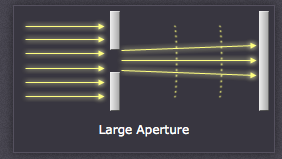
\includegraphics[scale=0.5]{images/1.png}
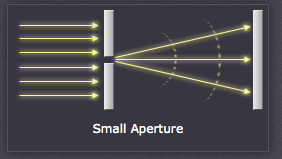
\includegraphics[scale=0.5]{images/2.png}

Since the divergent rays now travel different distances, some move out of phase and begin to interfere with each other — adding in some places and partially or completely canceling out in others. This interference produces a diffraction pattern with peak intensities where the amplitude of the light waves add, and less light where they subtract. If one were to measure the intensity of light reaching each position on a line, the measurements would appear as bands similar to those shown below.

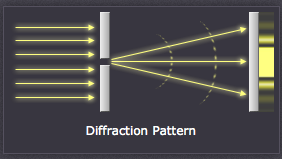
\includegraphics[scale=0.5]{images/3.png}

In general interference produces colorful effects due to the phase differences caused by a wave traversing thin media of different indices of refraction.

The effects of diffraction are often seen in everyday life. The most striking examples of diffraction are those that involve light; for example, the closely spaced tracks on a CD or DVD act as a diffraction grating to form the familiar rainbow pattern seen when looking at a disk

In optics, a diffraction grating is an optical component with a periodic structure, which splits and diffracts light into several beams travelling in different directions. The directions of these beams depend on the spacing of the grating and the wavelength of the light so that the grating acts as the dispersive element.

The relationship between the grating spacing and the angles of the incident and diffracted beams of light is known as the grating equation. 

FRAUENHOFER DIFFRACTION

\subsubsection{Radiometry}
Light is fundamentally a propagation form of enegry, so it is useful to define the SI unit of energy which is joule (J). To aid our intuition, let us describe radiometry in terms of collections of large numbers of photons. A photon can be considered as a quantum of light that has a position, direction of propagation and a wavelength $\lambda$ measured in nanometers. A photon travels in a certain speed, denoted by $v = \frac{c}{n}$, that depends only on the refractive index $n$ of the medium through which it propagates and the speed of light $c$. This allows us do define the frequency $f = \frac{c}{\lambda}$. The amount of energy $q$ carried by a photon is given by the following relationship: $q = hf= \frac{hc}{\lambda}$ where $h$ is the Plank's constant.

\myparagraph{Spectral Energy}
If there is a large collection of photons given, their total energy $Q = \sum_i q_i$ is the sum of energies of each photon $q_i$ within the collection. But how is the energy distributed across wavelenghts? One way in order to determine this distribution is to order all photons by their associated wavelength and then make a histogram from them. This is achieved by a discretization of their spectrum and combine all photons which will fall into the same interval, i.e. compute the sum for each interval from the energy of all their photons. By dividing such an interval by its length, denoted by $Q_\lambda$, we get a relatively scaled interval energy, which is called spectral energy and it is an intensive quantity. Intensive quantities can be thought of as density functions that tell the density of an extensive quantity at an infinitesimal point.

\myparagraph{Power}
Power is the estimated rate of energy production for light sources and is measured in the unit Watts, denoted by Q, which is another name for joules per second. Since power is a density over time, it is well defined even when energy production is varying over time. As with energy, we are really interested in the spectral power, measured in W/nm, denoted by $\Phi_\lambda$

\myparagraph{Irradiance}
The term irradiance comes into place when we are interested in \textit{how much light hits a given point}. In order to answer this question, we must make use of a density function. Let $\Delta A$ a finite area sensor that is smaller than the light field being measured. The spectral irradiance $E$ is just the power per unit area $\frac{\Delta \Phi}{\Delta A}$ which is 

\begin{equation}
 E = \frac{\Delta q}{\Delta A \Delta t \Delta \lambda}
\end{equation}

Thus the units of irradiance are $Jm^{-2}s^{-1}(nm)^{-1}$, the power per unit surface area.

\myparagraph{Radiance}

TODO: SHOW IMAGE: SOLID angle
$WIKI: http://en.wikipedia.org/wiki/Radiance$
$CG Slides 2012 - 6.shading$
$Book: Fundamentals of computer graphics$

Although irradiance tells us how much light is arriving at a point, it tells us little about the direction that light comes from. To measure something similar to what we see with our eyes we need to be able to associate the quantity \textit{how much light with a specific direction}. 

Radiance is a measure of the quantity of radiation that passes through or is emitted from a surface and falls within a given solid angle in a specified direction. Think of it as the energy carried along a narrow beam of light. 
This means radiance characterizes the total emission of reflectance. It indicates how much of the power emitted by a reflecting surface will be received by an optical system looking at the surface from some given angle of view. Formally, this leads us to the following definition of radiance: 

\begin{equation}
 L(\omega) = \frac{d^2 \Phi}{dA d\Omega cos(\theta)} \approx \frac{\Phi}{\Omega A cos(\theta)}
\end{equation}

where $L$ is the observed radiance in the unit energy per area per solid angle, which is $Wm^-2 sr^-1$ in direction $\omega$ which has an angle $\theta$ between the surface normal and $\omega$, $\Theta$ is the total flux or power emitted, $\theta$ is the angle between the surface normal and the specified direction, $A$ is the area of the surface and $\Omega$ is the solid angle in the unit steradian subtended by the observation or measurement.

It is useful to distinguish between radiance incident at a point on a surface and exitant from that point. Terms for these concepts sometimes used in the graphics literature are surface radiance $L_r$ for the radiance \textit{reflected} from a surface and field radiance $L_i$ for the radiance \textit{incident} at a surface.  

\myparagraph{BRDF}
The bidirectional reflectance distribution function, in short BRDF, denoted as $f_r(\omega_i, \omega_r)$ is a four dimensional function that defines \textit{how light is reflected at an opaque surface}. The function takes a negative directed incoming light direction, $\omega_{\text{i}}$, and outgoing direction, $\omega_{\text{r}}$ as input argument. Both are defined with respect to the surface normal $\mathbf{n}$.Hence A BRDF returns the ratio of reflected radiance exiting along $\omega_{\text{r}}$ to the irradiance incident on the surface from direction $\omega_{\text{i}}$, which is formally:
  
\begin{align}
  BRDF(\omega_i, \omega_r)
  & = f_r(\omega_i, \omega_r) \\
  & = \frac{dL_r(\omega_r)}{dE_i(\omega_i)} \\
  & = \frac{dL_r(\omega_r)}{L_i(\omega_i)cos(\theta_i)d\omega_i}
\end{align}

L is the reflected radiance, E is the irradiance and $\theta_{\text{i}}$ is the angle between $\omega_{\text{i}}$ and the surface normal, $\mathbf n$. The index $\text{i}$ indicates incident light, whereas the index $\text{r}$ indicates reflected light.

\myparagraph{Spectral Rendering}
In Computer Graphics, spectral rendering is where a scene's light transport is modeled considering the whole span of wavelengths instead of R,G,B values (still relating on geometric optic, which ignore wave phase). The motivation is that real colors of the physical world are spectrum; trichromatic colors are only inherent to Human Visual System.

In Computer Graphics, when talking about Spectral Rendering, we are refering to use the whole span of wavelengths instead just using RGB values in order for rendering a scene's light transport. The motivation for using the whole wavelength spectrum is due to the fact that trichromatic colors are only inherent to human visual system and therefore many phenomenons are poorly represented just using trichromy. 

\myparagraph{Color spaces}
In order to see how crucial the role human vision plays, we only have to look the the definition of color: 
\textit{Color is the aspect of visual perception by which an observer may distinguish differences between two structure-free filds of view of the same size and shape such as may be caused by differences in the spectral composition of the radiant energy concerned in the oberservation}. -  Wyszechki and Siles, 2000 mentioned in Computer Graphics Fundamentals Book. 

Each color can be represented by three numbers, for instance defined by (X,Y,Z) tristimulus values. However, its primaries are imaginary, meanung that is is not possible to construct a device that has three light sources (all positive) that can reprodue all colors in the visible spectrum. A large number of (X,Y,Z) values do not even correspond to a phyisical color. 

CIE 1931 RGB and CIE 1931 XYZ color spaces are the first mathematically defined color spaces. They were created by the International Commission on Illumination (CIE) in 1931.

The CIE's color matching functions $\overline{x}(\lambda)$, $\overline{y}(\lambda)$ and $\overline{z}(\lambda)$ are the numerical description of the chromatic response of the observer (described above). They can be thought of as the spectral sensitivity curves of three linear light detectors yielding the CIE tristimulus values X, Y and Z. Collectively, these three functions are known as the CIE standard observer.[9]

The tristimulus values for a color with a spectral power distribution $I(\lambda)$, are given in terms of the standard observer by:

\begin{align*}
    X= \int_{380}^{780} I(\lambda)\,\overline{x}(\lambda)\,d\lambda \\
    Y= \int_{380}^{780} I(\lambda)\,\overline{y}(\lambda)\,d\lambda \\
    Z= \int_{380}^{780} I(\lambda)\,\overline{z}(\lambda)\,d\lambda
\end{align*}

where $\lambda$, is the wavelength of the equivalent monochromatic light (measured in nanometers).

It is not possible to build a display that corresponds to CIE XYZ, for this reasons it is necessary to design  other color spaces, which are phyiscal realizable, offers efficient encoding, are perceptual uniform and have an intuitive color specification. 

There are simple conversions between XYZ color space to any other color space defined, as linear transfromations.


\subsubsection{Signal Processing Basics}
A signal is a function that conveys information about the behavior or attributes of some phenomenon.
In the physical world, any quantity exhibiting variation in time or variation in space (such as an image) is potentially a signal that might provide information on the status of a physical system, or convey a message between observers

\myparagraph{Fourier Transformation}
The Fourier-Transform is a mathematical tool which allows to transform a given function or rather a given signal from defined over a time- (or spatial-) domain into its corresponding frequency-domain.
 
Let $f$ an measurable function over $\mathds{R}^n$. Then, the continnous Fourier Transformation(\textbf{FT}), denoted as $\mathcal{F}\{f\}$ of $f$ is defined as, ignoring all constant factors in the formula:
 
\begin{equation}
  \mathcal{F}_{FT}\{f\}(w) = \int_{\mathds{R}^n} f(x)e^{-iwt} dt
\end{equation}

whereas its inverse transform is defined like the following which allows us to obtain back the original signal:

\begin{equation}
  \mathcal{F}_{FT}^{-1}\{f\}(w) = \int_{\mathds{R}} \mathcal{F}\{w\}e^{iwt} dt
\end{equation}

An usual identity for $w$ is the the so called angular with $w = \frac{2 \pi}{T} = 2 \pi v_f$ where T is the period, $v_f$ the frequency.

By using Fourier Analysis, which is the approach to approximate any function by sums of simpler trigonometric functions, we gain the so called Discrete Time Fourier Transform (in short \textbf{DTFT}). The DTFT operates on a discrete function. Usually, such an input function is often created by digitally sampling a continnous function. The DTFT itself is operation on a discretized signal on a continnous, periodic frequency domain and looks like the following:

\begin{equation}
  \mathcal{F}_{DTFT}\{f\}(w) = \sum_{-\infty}^{\infty} f(x) e^{-iwk}
\end{equation}

We can further discretize the frequency domain and will get then the Discrete Fourier Transformation (in short \textbf{DFT}) of the input signal:

\begin{equation}
  \mathcal{F}_{DFT}\{f\}(w) = \sum_{n=0}^{N-1} f(x) e^{-iw_{n}k}
\end{equation}

Where the angular frequency $w_n$ is defined like the following $w_n = \frac{2\pi n}{N}$ and N is the number of samples within an equidistant periode sampling.

\myparagraph{Convolution}
The convolution $f*g$ of two functions $f$, $g$$\colon \mathds{R}^n \to \mathds{C} $ is defined as:  
\begin{equation}
  \mathcal (f*g)(t) = \int_{\mathds{R}^n} f(t)g(t-x) dx
\end{equation}

Note that the Fourier transform of the convolution of two functions is the product of their Fourier transforms. This is equivalent to the fact that Convolution in spatial domain is equivalent to multiplication in frequency domain. Therefore, the inverse Fourier transform of the product of two Fourier transforms is the convolution of the two inverse Fourier transforms

\myparagraph{Taylor Series}
Taylor series is a representation of a function as an infinite sum of terms that are calculated from the values of the function's derivatives at a single point.

The Taylor series $\mathcal T$ of a real or complex-valued function ƒ(x) that is infinitely differentiable at a real or complex number $a$ is the power series:
\begin{equation}
  \mathcal T(f;a)(x) = \sum_{n=0}^{\infty} \frac{f^{n}(a)}{n!}(x-a)^n
\end{equation}


\subsection{Thesis Basis: J.Stam's Paper about Diffraction Shader}
In his paper about Diffraction Shader, J. Stam derives a BRDF which is modeling the effect of diffraction for various analytical anisotropic reflexion models relying on the so called scalar wave theory of diffraction for which a wave is assumed to be a complex valued scalar. 
It's noteworthy, that Stam's BRDF formulation does not take into account the polarization of the light. Fortunately, light sources like sunlight and light bulbs are unpolarized. 

A further assumption in Stam's Paper is, the emanated waves from the source are stationary, which implies the wave is a superposition of independent monochromatic waves. This implies that each wave is associated to a definite wavelangth lambda. However, sunlight once again fulfills this fact.

In our simulations we will always assume we have given a directional light source, i.e. sunlight. Hence, Stam's model can be used for our derivations.

Based on his these previous assumptions and applying Stam starts his derivations by applying the so called Kirchhoff integral, which is relating the reflected field to the incoming field. This equation is a formalization of Huygen’s well-known principle that states that if one knows the wavefront at a given moment, the wave at a later time can be deduced by considering each point on the first wave as the source of a new disturbance, i.e. once the field  $\psi_1 =  e^{ik\mathbf{x} \cdot \mathbf{s}\mathbf{s}}$ on the surface is known, the field everywhere $\psi_2$ else away from the surface can be computed.
More precisely, we want to compute the wave $\psi_2$ equal to the reflection of an incoming planar monochromatic wave $\psi_1 = e^{ik \omega_i * x}$  traveling in the direction $\omega_i$ from a surface S to the light source. Mathematically this can be formulized the following:

\begin{equation}
  \psi_2 = \frac{i k e^{i K R}}{4 \pi R}(F\mathbf{v}-\mathbf{p}) \cdot \int_{S} \hat{\mathbf{n}} e^{ik\mathbf{v} \cdot \mathbf{s} d\mathbf{s}}
\end{equation}


In applied optics, when dealing with scattered waves, one does use differential scattering cross-section rather than defining a BRDF which has the following identitiy: 

\begin{equation}
    \sigma^0 = 4 \pi \lim_{R \to \infty} R^2 \frac{\langle \left|\psi_2\right|^2\rangle}{\langle \left|\psi_1\right|^2\rangle}
\end{equation}

where R is the distance from the center of the patch to the receiving point $x_p$, $\hat{\mathbf{n}}$ is the normal of the surface at s and the vectors:

The relationship between the BRDF and the scattering cross section can be shown to be equal to 

\begin{equation*}
 BRDF = \frac{1}{4\pi}\frac{1}{A}\frac{\sigma^0}{cos(\theta_i)cos(\theta_r)}
\end{equation*}


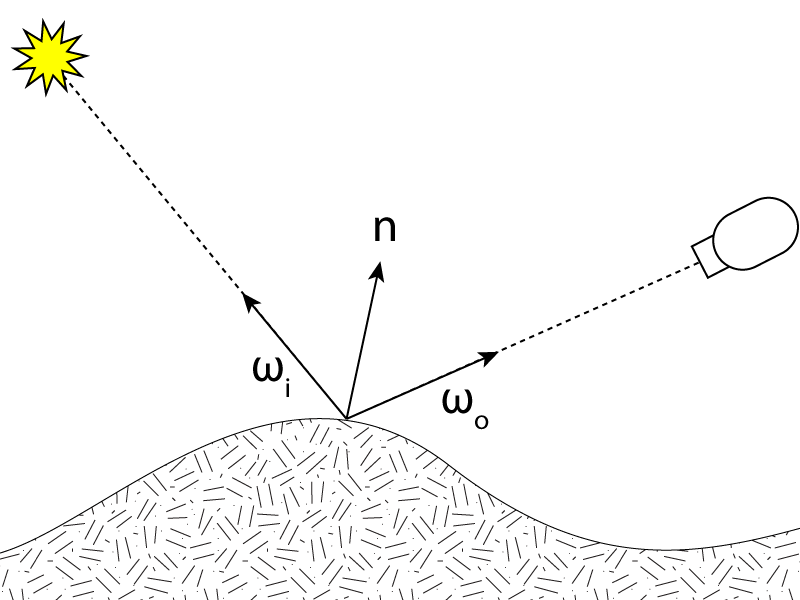
\includegraphics[scale=0.25]{images/brdfdiagram.png}
where $\omega_i$ is the incident unit direction vector and $\omega_r$ is the reflected unit direction vector.

The components of vector resulting by the difference between these direction vectors:

\begin{equation*}
  -\omega_i - \omega_r = (u,v,w)
\end{equation*}

are used in almost every step of his derivations.

Stam formulates for a hightfield auxilary function $p(x,y) = e^{iwkh(x,y)}$ where $w = -(cos(\theta_i)+cos(\theta_r))$ and $\theta_i$ and $\theta_r$ are the angles of incident and reflected directions with the surface normal and the wavenumber $k=\frac{2\pi}{\lambda}$


During his derivations, Stam provides a analytical representation for the Kirchhoff integral by using his assumptions. He restricts himself to the reflexion of waves on a surface represented by a heightfield $h(x,y)$ with the assumption that the surface is defined as an elevation over the (x,y)-plane using the surface plane approximation.
This will lead him to the follwoing identity for the Kirchhoff integral:

\begin{equation}
    \mathbf{I}(ku, kv) = \int \int \frac{1}{ikw}(-p_x, -p_y, ikwp) 
\end{equation}


We the observation that the integral is a Fourier transform by $-iku$ and $-ikv$
which will lead us to his final derivation, using the identity of BRDF, and computing the limes:

\begin{equation} \label{eq:mainstam}
    BRDF_{\lambda}(\omega_i, \omega_r) = \frac{k^2 F^2 G}{4\pi^2 A w^2} \langle \left|P(ku, kv)\right|^2\rangle
\end{equation}

Where $BRDF_{\lambda}(\omega_i, \omega_r)$ is BRDF where wavelength $\lambda$ $\omega_i$ and $\omega_r$ are incident and reflected normalized directions vectors, pointing away from the given surface. Which can be written, using the fourier transform (FT) $P(u,v) = F(p)(u,v)$, as:
$BRDF_{\lambda}(\omega_i, \omega_r) = \frac{F^2 G}{\lambda^2 A w^2}abs(P(\frac{u}{\lambda},\frac{v}{\lambda}))^2$ where F represents the Fresnel term, uv,v,w are derived from the incident and reflected directions as $(u,v,w) = -\omega_i - \omega_r$, abs(P) represents the expected valuess of a random variable X and A is an area of integration on the surface that is considered to contribute to diffraction, G is the geometry term which is $G   =\frac{(1 + \omega_i \cdot \omega_r)^2}{cos(\theta_i)cos(\theta_r)}$

and $P(x,y)$ is the Fourier Transform (FT) of the function $p(x,y)$ from above.

\subsection{Derivations}
\subsubsection{BRDF formulation}
Lets assume we have given an incoming light source with solid angle $\omega_i$, $\theta{_i}$ is its angle of incidence, $\omega_r$ is the solid angle for the reflected light, $\lambda$ wavelength, $\Omega$ is the hemisphre we of integration for the incomming light. Then, we are able to formulate a BRDF by using its definiton:  

\begin{align*}
f_r(\omega_i, \omega_r) = \frac{dL_r(\omega_r)}{L_i(\omega_i)cos(\theta_i)d\omega_i} \\
=> f_r(\omega_i, \omega_r) L_i(\omega_i)cos(\theta_i)d\omega_i = dL_r(\omega_r) \\
=> \int_{\Omega}f_r(\omega_i, \omega_r) L_i(\omega_i)cos(\theta_i)d\omega_i = \int_{\Omega}dL_r(\omega_r) \\
=> L_r(\omega_r) = \int_{\Omega}f_r(\omega_i, \omega_r) L_i(\omega_i)cos(\theta_i)d\omega_i
\end{align*}

The last equation is the so called rendering equation.
We assume further, that our incident light is a directional, unpolarized light source like sunlight and therefore its radiance is given as 

\begin{equation}
 L_{\lambda}(\omega)=I(\lambda)\delta(\omega-\omega_i)
\end{equation}

where $I(\lambda)$ is the intensity of the relative spectral power for the wavelength $\lambda$. 
Since all light rays are parallel whenever we are provided by a directional light source and we can think of radiance as a measure of the light emitted from a particular surface location into a particular direction, above's radiance identity will follow immediately. 
By plugging this identity into our current rendering equation, we will get:

\begin{align}
L_{\lambda}(w_r) 
& = \int_{\Omega} BRDF_{\lambda}(\omega_i, \omega_r) L_{\lambda}(\omega_i) cos(\theta_i) d\omega_i \\
& = BRDF_{\lambda}(\omega_i, \omega_r) I(\lambda) cos(\theta_i)
\end{align}

where $L_{\lambda}(\omega_i)$ is the incomming radiance and $L_{\lambda}(\omega_r)$ is the radiance reflected by given surface
Note that above's integral vanishes since $\delta(\omega-\omega_i)$ is only equal one if and only if $\omega = \omega_i$.

For the $BRDF(\omega_i, \omega_r)$ we are going to use Stam's main derivation $~\eqref{eq:mainstam}$ applying the fact that the wavenumber is equal $k=\frac{2\pi}{\lambda}$:

\begin{align*}
BRDF(\omega_i, \omega_r) 
& = \frac{k^2 F^2 G}{4\pi^2 A w^2} \langle \left|P(ku, kv) \right|^2\rangle \\
& = \frac{k^2 F^2 (1 + \omega_i \cdot \omega_r)^2}{cos(\theta_i)cos(\theta_r) 4\pi^2 A w^2} \langle \left|P(ku, kv)  \right|^2\rangle \\
& = \frac{4 \pi^2 F^2 (1 + \omega_i \cdot \omega_r)^2}{cos(\theta_i)cos(\theta_r) 4\pi^2 A \lambda^2 w^2} \langle \left|P(ku, kv)  \right|^2\rangle \\
& = \frac{F(w_i, w_r)^2 (1 + \omega_i \cdot \omega_r)^2}{cos(\theta_i)cos(\theta_r) A \lambda^2 w^2} \langle \left|P(ku, kv)  \right|^2\rangle
\end{align*}

going back to the definition of $(u,v,w)= -\omega_i - \omega_r$ and using spherical coordinates, we get for $w$ the following identity $w = -\omega_i - \omega_r = -(\omega_i + \omega_r) = -(cos(\theta_i)+cos(\theta_r))$ and therefore $w^2$ is equal $(cos(\theta_i)+cos(\theta_r))^2$
This new fact will allow us to get even further:

\begin{align*}
L_{\lambda}(\omega_r) 
& = \frac{F(\omega_i, \omega_r)^2 (1 + \omega_i \cdot \omega_r)^2}{A \lambda^2 cos(\theta_i)cos(\theta_r)  (cos(\theta_i)+cos(\theta_r))^2} \langle \left|P_{cont}(\frac{2\pi u}{\lambda}, \frac{2\pi v}{\lambda})  \right|^2\rangle cos(\theta_i) I(\lambda) \\
& = I(\lambda) \frac{F(\omega_i, \omega_r)^2 (1 + \omega_i \cdot \omega_r)^2}{\lambda^2 A (cos(\theta_i)+cos(\theta_r))^2 cos(\theta_r)} \langle \left|P_{cont}(\frac{2\pi u}{\lambda}, \frac{2\pi v}{\lambda})  \right|^2\rangle \\
& = I(\lambda) \frac{F(\omega_i, \omega_r)^2 (1 + \omega_i \cdot \omega_r)^2}{\lambda^2 A (cos(\theta_i)+cos(\theta_r))^2 cos(\theta_r)} \langle \left|T_0^2 P_{dtft}(\frac{2\pi u}{\lambda}, \frac{2\pi v}{\lambda})  \right|^2\rangle
\end{align*}

$P_{cont}$ denotes the continuous inverse Fourier-Transform for the Taylor-Series of our heightfield representing the nano-scaled surface structure, i.e. $P(k,l) = \mathcal{F}^{-1}\{p\}(k,l)$ and $P_{dtft}$ is the inverse Discrete Time Fourier Transform of $p(x,y) = e^{ikwh(x,y)}$. Furthermore $T_0$ the sampling distance for the discretization of $p(x,y)$ assuming equal and uniform sampling in both dimensions $x,y$.

\subsubsection{Relative BRDF}
In this section we are going to explain how to scale our BRDF formulation such that all of its possible output values are mapped into the range $\left[0,1\right]$. Such a relative BRDF formulation will ease our life for later rendering puposes since usually color values are within the range $\left[0,1\right]$, too. Furthermore, this will allow us to properly blend the resulting illumination caused by diffraction with a texture map.

Let us examine what $L_\lambda(\omega_r)$ will be for $\omega_r = \omega_0 := (0,0,*)$ i.e. specular reflection case, denoted as $L_\lambda^{spec}(\omega_0)$. 

When we know the expression for $L_\lambda^{spec}(\omega_0)$ we would be able to compute the relative reflected radiance for our problem by simply dividing $L_\lambda(\omega_r)$ by $L_\lambda^{spec}(\omega_0)$, denoted as 

\begin{equation}
    \rho_\lambda(\omega_i,\omega_r) = \frac{L_\lambda(\omega_r)}{L_\lambda^{spec}(\omega_0)}
\end{equation}

But first, let us derive the following expression:

\begin{align*}
L_\lambda^{spec}(\omega_0) 
& = I(\lambda) \frac{F(\omega_0, \omega_0)^2 (1+\colvec[0]{0}{1}\cdot\colvec[0]{0}{1})^2}{\lambda^2 A (cos(0)+cos(0))^2 cos(0)} \langle \left|T_0^2 P_{dtft}(0,0)  \right|^2\rangle \\
& = I(\lambda) \frac{F(\omega_0, \omega_0)^2 (1+1)^2}{\lambda^2 A (1+1)^2 1}\left| T_0^2 N_{sample} \right|^2 \\
& = I(\lambda) \frac{F(\omega_0, \omega_0)^2}{\lambda^2 A}\left| T_0^2 N_{sample} \right|^2 
\end{align*}

Where $N_{samples}$ is the number of samples of the DTFT.

Thus, we can plug our last derived expression into the definition for the relative reflectance radiance in the direction $w_r$ and will get:

\begin{align*}
\rho_\lambda(\omega_i,\omega_r)
& = \frac{L_\lambda(\omega_r)}{L_\lambda^{spec}(\omega_0)} \\
& = \frac{I(\lambda) \frac{F(\omega_i, \omega_r)^2 (1 + \omega_i \cdot \omega_r)^2}{\lambda^2 A (cos(\theta_i)+cos(\theta_r))^2 cos(\theta_r)} \langle \left|T_0^2 P_{dtft}(\frac{2\pi u}{\lambda}, \frac{2\pi v}{\lambda}) \right|^2\rangle}{I(\lambda) \frac{F(\omega_0, \omega_0)^2}{\lambda^2 A}\left| T_0^2 N_{sample} \right|^2 } \\
& = \frac{F^2(\omega_i,\omega_r)(1 + \omega_i \cdot \omega_r)^2}{F^2(\omega_0,\omega_0)(cos(\theta_i)+cos(\theta_r))^2 cos(\theta_r)} \langle \left|\frac{P_{dtft}(\frac{2\pi u}{\lambda}, \frac{2\pi v}{\lambda})}{N_{samples}}\right|^2\rangle
\end{align*}

for simplification and a better overview, let us introduce the following expression, the so called gain-factor:

\begin{equation} \label{eq:cfact}
    C(\omega_i,\omega_r) = \frac{F^2(\omega_i,\omega_r)(1 + \omega_i \cdot \omega_r)^2}{F^2(\omega_0,\omega_0)(cos(\theta_i)+cos(\theta_r))^2 cos(\theta_r) N_{samples}^2}
\end{equation}

Using this substitute, we will end up with the following expression for the relative reflectance radiance:

\begin{equation}
\rho_\lambda(\omega_i,\omega_r) =  C(\omega_i,\omega_r) \langle \left|P_{dtft}(\frac{2\pi u}{\lambda}, \frac{2\pi v}{\lambda})\right|^2\rangle
\end{equation}

Using the previous definition for the relative reflectance radiance 

\begin{equation}
 \rho_\lambda(\omega_i,\omega_r) = \frac{L_\lambda(\omega_r)}{L_\lambda^{spec}(\omega_0)} 
\end{equation}

which we can rearrange to the expression 

\begin{equation}
L_\lambda(\omega_r) = \rho_\lambda(\omega_i,\omega_r)L_\lambda^{spec}(\omega_0)
\end{equation}

Let us choose $L_\lambda^{spec}(w_0) = S(\lambda)$ such that is has the same profile as the relative spectral power distribuation of CIE Standard Illuminant $D65$. Further, when integration over $\lambda$ for a specular surface we should get $CIE_{XYZ}$ values corresponding to the white point for $D65$ 
The corresponding tristimulus values using CIE colormatching functions for the $CIE_{XYZ}$ values look like:

\begin{equation}
X = \int_{\lambda}L_\lambda(\omega_r)\overline{x}(\lambda)d\lambda
\end{equation} 

\begin{equation}
Y = \int_{\lambda}L_\lambda(\omega_r)\overline{y}(\lambda)d\lambda
\end{equation}

\begin{equation}
Z = \int_{\lambda}L_\lambda(\omega_r)\overline{z}(\lambda)d\lambda
\end{equation}

where $\overline{x}$, $\overline{y}$, $\overline{z}$ are the color matching functions

Using our last finding for $L_\lambda(\omega_r)$ with the definition for the tristimulus values we can actually derive an expression for computing the colors for our BRDF formula. 
Since X, Y, Z are defined similarly, it satisfies to derive an explicit expression for just one tristimulus term, for example X. The other two will look the same, except the we have to replace all X with Y or Z respectively. Therefore, we get:

\begin{align*}
X 
& =\int_{\lambda}L_\lambda(\omega_r)\overline{x}(\lambda)d\lambda \\
& =\int_{\lambda}\rho_\lambda(\omega_i,\omega_r)L_\lambda^{spec}(\omega_0) \overline{x}(\lambda)d\lambda \\
& =\int_{\lambda}\rho_\lambda(\omega_i,\omega_r) S(\lambda) \overline{x}(\lambda)d\lambda \\
& =\int_{\lambda} C(\omega_i,\omega_r) \langle \left|P_{dtft}(\frac{2\pi u}{\lambda}, \frac{2\pi v}{\lambda})\right|^2\rangle S(\lambda) \overline{x}(\lambda)d\lambda \\
& = C(\omega_i,\omega_r) \int_{\lambda} \langle \left|P_{dtft}(\frac{2\pi u}{\lambda}, \frac{2\pi v}{\lambda})\right|^2\rangle S(\lambda) \overline{x}(\lambda)d\lambda \\
& = C(\omega_i,\omega_r) \int_{\lambda} \langle \left|P_{dtft}(\frac{2\pi u}{\lambda}, \frac{2\pi v}{\lambda})\right|^2\rangle S_x(\lambda)d\lambda
\end{align*}

Where we used the definition $S_x(\lambda)\overline{x}(\lambda)$ in the last step.

\subsubsection{Taylor approximation for BRDF}
In this section, we will deliver an approximation for the inverse Fourier Tranformation of Stam's auxilary function p(x,y)s. This derivation will rely on the definition of Taylor Series expansion. Further, we will provide an error bound for our approximation approach for a given number of iterations. Last, we will extend our current BRDF formula by the findings derived within this section.

Given $p(x,y)=e^{ikwh(x,y)}$ form Stam's Paper where h(x,y) is a given heightfield. Let be y real or even complex value, and lets consider the power series for the the exponential function 
\begin{equation*}
  e^{t}=1+t+\frac{t^{2}}{2!}+\frac{t^{3}}{3!}+...=\sum_{n=0}^{\infty}\frac{t^{n}}{n!}
\end{equation*}

Let us define $t := t(x,y) = ikwh(x,y)$ where $i$ is the imaginary number.
For simplification, let us denote $h(x,y)$ as $h$. Then it follows by our previous
stated identities: 

\begin{align*}
 e^{t}
 &=1+(ikwh)+\frac{1}{2!}(ikwh)^{2}+\frac{1}{3!}(ikwh)^{3}+... \\
 &=\sum_{n=0}^{\infty}\frac{(ikwh)^{n}}{n!}.
\end{align*}

Hence it holds $p(x,y)=\sum_{n=0}^{\infty}\frac{(ikwh(x,y))^{n}}{n!}.$

Let us now compute the Fourier Transformation of p(x,y) form above:
\begin{align*}
  \mathcal{F}\left\{ p\right\}(u,v)
  & =\mathcal{F}\left\{ \sum_{n=0}^{\infty}\frac{(ikwh)^{n}}{n!}.\right\}(u,v) \\
  & =^{\mathcal{F}\, lin\, Operator}\sum_{n=0}^{\infty}\mathcal{F}\left\{ \frac{(ikwh)^{n}}{n!}\right\}(u,v) \\
  & =\sum_{n=0}^{\infty}\frac{(ikw)^{n}}{n!}\mathcal{F}\left\{ h{}^{n}\right\}(u,v)
\end{align*}

Hence it follows: $P(\alpha,\beta)=\sum_{n=0}^{\infty}\frac{(ikw)^{n}}{n!}\mathcal{F}\left\{ h{}^{n}\right\} (\alpha,\beta)$ for which $\mathcal{F}_{FT}\left\{ h{}^{n}\right\} (u,v)$.

Next we are going to look for an $N\mathbb{\in N}$ such that 
\begin{equation*}
 \sum_{n=0}^{N}\frac{(ikwh)^{n}}{n!}\mathcal{F}\left\{ h{}^{n}\right\} (\alpha,\beta) \approx P(\alpha,\beta) 
\end{equation*}

is a good approximation. But first the following two facts have to be proven:

\begin{enumerate}
\item Show that there exist such an $N\mathbb{\in N}$s.t the approximation
holds true.
\item Find a value for B s.t. this approximation is below a certain error
bound, for example machine precision $\epsilon$. 
\end{enumerate}

\myparagraph{Proof Sketch of 1.}

By the \textbf{ratio test} (see \textbf{{[}1{]}}) 
It is possible to show that the series $\sum_{n=0}^{N}\frac{(ikwh)^{n}}{n!}\mathcal{F}\left\{ h{}^{n}\right\} (\alpha,\beta)$ converges absolutely:

\textbf{Proof}: Consider $\sum_{k=0}^{\infty}\frac{y^{n}}{n!}$ where
$a_{k}=\frac{y^{k}}{k!}$. By applying the definition of the ratio test for this series it follows: 
\begin{equation*}
 \forall y:limsup_{k\rightarrow\infty}|\frac{a_{k+1}}{a_{k}}|=limsup_{k\rightarrow\infty}\frac{y}{k+1}=0 
\end{equation*}

Thus this series converges absolutely, no matter what value we will
pick for y.

\myparagraph{Part 2: Find such an N}
Let $f(x)=e^{x}$. We can formulate its Taylor-Series, stated above.
Let $P_{n}(x)$denote the n-th Taylor-Polinomial, 
\begin{equation*}
 P_{n}(x)=\sum_{k=0}^{n}\frac{f^{(k)}(a)}{k!}(x-a)^{k}
\end{equation*}
where $a$ is our developing point (here a is equal zero). 

We can define the error of the n-th Taylor-Polinomial to be $E_{n}(x)=f(x)-P_{n}(x)$.
the error of the n-th Taylor-Polinomial is difference between the value of the function and the Taylor polinomial
This directly implies $|E_{n}(x)|=|f(x)-P_{n}(x)|$. By using the Lagrangien Error Bound it follows: 

\begin{equation*}
 |E_{n}(x)|\leq\frac{M}{(n+1)!}|x-a|^{n+1} 
\end{equation*}

with $a=0$, where \textbf{M} is some value satisfying $|f^{(n+1)}(x)|\leq M$ on the interval $I=[a,x]$. Since we are interested in an upper bound of the error and since \textbf{a} is known, we can reformulate the interval as $I=[0,x_{max}]$, where 

\begin{equation*}
 x_{max} = \|i\| k_{max} w_{max} h_{max}
\end{equation*}

We are interested in computing an error bound for $e^{ikwh(x,y)}$. Assuming the following parameters and facts used within Stam's Paper: 

\begin{itemize}
\item Height of bump: 0.15micro meters
\item Width of a bump: 0.5micro meters
\item Length of a bump: 1micro meters
\item $k=\frac{2\pi}{\lambda}$ is the wavenumber, $\lambda\in[\lambda_{min,}\lambda_{max}]$ and
thus $k_{max}=\frac{2\pi}{\lambda_{min}}$. Since $(u,v,w) = -\omega_i - \omega_r$ and both are unit direction vectors, 
each component can have a value in range {[}-2, 2{]}.
\item for simplification, assume$[\lambda_{min,}\lambda_{max}]=[400nm,700nm].$

\end{itemize}

We get:  

\begin{align*}
x_{max}
 &= \|i\|*k_{max}*w_{max}*h_{max} \\
 &= k_{max}*w_{max}*h_{max} \\
 &=2*(\frac{2\pi}{4*10^{-7}m})*1.5*10^{-7} \\
 &=1.5\pi
\end{align*}

and it follows for our intervall $I=[0,1.5\pi]$. 

Next we are going to find the value for $M$. Since the exponential function is monotonically growing (on the interval I) and the derivative of the \textbf{exp} function is the exp function itself, we can find such an $M$: 
\begin{align*}
 M
 &=e^{x_{max}} \\
 &=exp(1.5\pi)
\end{align*}

and $|f^{(n+1)}(x)|\leq M$ holds. With 

\begin{align*}
|E_{n}(x_{max})|
 &\leq\frac{M}{(n+1)!}|x_{max}-a|^{n+1} \\
 &= \frac{exp(1.5\pi)*(1.5\pi)^{n+1}}{(n+1)!}
\end{align*}

we now can find a value of $n$ for a given bound, i.e. we can find an value of $N\mathbb{\in N}$ s.t. $\frac{exp(1.5\pi)*(1.5\pi)^{N+1}}{(N+1)!}\leq\epsilon$.
With Octave/Matlab we can see: 
\begin{itemize}
\item if N=20 then $\epsilon\approx2.9950*10^{-4}$
\item if N=25 then $\epsilon\approx8.8150*10^{-8}$
\item if N=30 then $\epsilon\approx1.0050*10^{-11}$
\end{itemize}

With this approach we have that $\sum_{n=0}^{25}\frac{(ikwh)^{n}}{n!}\mathcal{F}\left\{ h{}^{n}\right\} (\alpha,\beta)$ is
an approximation of $P(u,v)$ with error $\epsilon\approx8.8150*10^{-8}$. This means we can precompute 25 Fourier Transformations in order to approximate P(u,v) having an error $\epsilon\approx8.8150*10^{-8}$. 

Using now our approximation for $P_{dtft} = \mathcal{F}^{-1}\{p\}(u,v)$ for the tristumulus value X, we will get:

\begin{align*}
X 
& = C(w_i,w_r) \int_{\lambda} \langle \left|P_{dtft}(\frac{2\pi u}{\lambda}, \frac{2\pi v}{\lambda})\right|^2\rangle S_x(\lambda)d\lambda \\
& = C(w_i,w_r) \int_{\lambda} \left| \sum_{n=0}^N \frac{(wk)^n}{n!} \mathcal{F}^{-1}\{i^n h^n\}(\frac{2\pi u}{\lambda}, \frac{2\pi v}{\lambda})\right|^2 S_x(\lambda)d\lambda
\end{align*}

\subsubsection{Sampling: Gaussian Window}
Practically, we cannot compute the DTFT numerically due to finite computer arithmetic, since $w$ is a continuous function for the DTFT. 
The DFT of a discrete heightfield patch is equivalent to the DTFT of an infinitely periodic function consisting of replicas of the same discrete patch. By windowing with a window function that is zero outside the central replica, the convolution of either the DFT or the DTFT of heightfield with the fourier transfrom of the window becomes equivalent.

Let $window_g$ denote the gaussian window with $4\sigma_s$ $\mu m$ where $\sigma_f = \frac{1}{2\pi\sigma_s}$
let us further substitute $\mathbf{t(x,y)}=i^n h(x,y)^n$

\begin{equation}
\mathcal{F}_{dtft}^{-1}\{\mathbf{t}\}(u,v) = \mathcal{F}_{fft}^{-1}\{\mathbf{t}\}(u,v)window_g(\sigma_f)
\end{equation} 

Therefore we can deduce the following expression from this:

\begin{align*}
\mathcal{F}_{dtft}^{-1}\{\mathbf{t}\}(u,v)
& = \int_{-\infty}^{\infty} \int_{-\infty}^{\infty} {F}_{fft}^{-1}\{\mathbf{t}\}(w_u,w_v) \phi(u-w_u, v-w_v) dw_u dw_v \\
& = \int_{-\infty}^{\infty} \int_{-\infty}^{\infty} \sum_i \sum_j {F}_{fft}^{-1}\{\mathbf{t}\}(w_u,w_v) \\ 
& \quad \quad \delta(w_u-w_i, w_v-w_j)\phi(u-w_u, v-w_v) dw_u dw_v \\
& = \sum_i \sum_j \int_{-\infty}^{\infty} \int_{-\infty}^{\infty}  {F}_{fft}^{-1}\{\mathbf{t}\}(w_u,w_v) \\
& \quad \quad \delta(w_u-w_i, w_v-w_j)\phi(u-w_u, v-w_v) dw_u dw_v \\
& = \sum_i \sum_j {F}_{fft}^{-1}\{\mathbf{t}\}(w_u,w_v) \phi(u-w_u, v-w_v)
\end{align*}

where 

\begin{equation} \label{eq:gaussweight}
 \phi(x,y) = \pi e^{-\frac{x^2 + y^2}{2\sigma_{f}^2}}
\end{equation} 

\subsubsection{Final Expression}
As the last step of our series of derivations, we plug all our findings together to one big equation in order to compute the color for each pixel on our mesh in the $CIE_XYZ$ colorspace:

For a given heigh-field $h(x,y)$, representing a small patch of the nano-structure of our surface, the resulting $CIE_{XYZ}$ caused by the effect of diffraction can be computed like the following: 

Let $P(u,v,\lambda) = {F}_{fft}^{-1}\{i^n h^n\}(\frac{2\pi u}{\lambda},\frac{2\pi v}{\lambda})$

\begin{equation}
\begin{split}
\colvec[X]{X}{Z}& = C(\omega_i,\omega_r) \int_{\lambda} \sum_{n=0}^N  \frac{(wk)^n}{n!} \sum_{(r,s) \in \mathcal{N}_1(u,v)} \left| P_{\lambda}(u-w_r,v-w_s) \right|^2 \\
& \quad \quad  \phi(u-w_r, v-w_s) \colvec[S_x(\lambda)]{S_y(\lambda)}{S_z(\lambda)}d\lambda
\end{split}
\end{equation}

where $\phi(x,y) = \pi e^{-\frac{x^2 + y^2}{2\sigma_{f}^2}}$ is the gaussian window.
where $w_s$ and $w_r$ are ... explain them

\subsubsection{Aplitude smooting}
REASON FOR WHICH CASE THIS CAN BE USED, ADD AN IMAGE OF BOXFUNCTION
The approach introduced within this section is an alternative to the gaussian window approach.
Let us consider the so called 1-dimensional Box-function with length $T$ which is defined as the following: 

$
Box(x) =
\left\{
	\begin{array}{ll}
		1  & \mbox{if } x \leq T \\
		0 & \mbox{if } else
	\end{array}
\right.
$

We assume, that our given heighfield can be represented as a 2-dimensional box-function. 
Note that we can use any explicit given constrainted 2-dimensional function and will get some identities like
we get from the box-function.
 
Further we are assuming that we can model the overall surface be assuming this heighfield being distributed in a periodic manor.
Therfore, the whole surface can be represented like this $f(x) = \sum_{n=0}^{N} Box(x+nT_1, y+mT_2)$ assuming the given heighfield has the dimensions $T_1$ by $T_2$. But let us first consider the 1-dimensional Box-function case before deriving an identity for the Fourier transform of our 2-dimensional Box-function, i.e. the fourier transform of our heighfield. 

Note: A function $f$ periodic with periode $T$ means: $\forall x \in \mathcal{R}: Box(x) = Box(x+T)$

A so called bump can be represented by our 1-dimensional Box-function. We assume periodicity which is equaivalent to:   
$f(x) = \sum_{n=0}^{N} Box(x+nT)$

We are insterested in the 1-dimensional inverse Fourier transform of the 1-dimensional Box-function:

\begin{align*}
\mathcal{F}^{-1}\{f\}(w)
& =\int f(x) e^{iwx}dx\\
& =\int_{-\infty}^{\infty} \sum_{n=0}^{N} Box(x+nT) e^{iwx}dx\\
& =\sum_{n=0}^{N} \int_{-\infty}^{\infty} Box(x+nT) e^{iwx}dx
\end{align*}

Next, apply the following substituation $x+nT = y$ which will lead us to:

\begin{gather*}
x=y-nT\\
dx=dy
\end{gather*} 

Plugging this substituation back to the equation from above we will get 

\begin{align*}
\mathcal{F}^{-1}\{f\}(w)
& =\int f(x) e^{iwx}dx\\
& =\sum_{n=0}^{N} \int_{-\infty}^{\infty} Box(y) e^{iw(y-nT)}dy \\
& =\sum_{n=0}^{N} e^{-iwnT} \int_{-\infty}^{\infty} Box(y) e^{iwy}dy \\
& =\sum_{n=0}^{N} e^{-iwnT} \mathcal{F}\{f\}(w) \\
& =\mathcal{F}^{-1}\{f\}(w) \sum_{n=0}^{N} e^{-iwnT}  
\end{align*}

We used the fact that the term $e^{-iwnT}$ is a constant when integrating along $dy$ and the identity for the inverse Fourier transform of the Box function. Next, let us consider $\sum_{n=0}^N e^{-uwnT}$ further:

\begin{align*}
\sum_{n=0}^N e^{-uwnT}
& =\sum_{n=0}^N (e^{-uwT})^n \\
& =\frac{1-e^{iwT(N+1)}}{1-e^{-iwT}}
\end{align*}

We recognize the geometric series identity for the left-handside of this equation. Since our series is bounded we can derive our right-handside.

Since $e^{-ix}$ is a complex number and every complex number can be written in its polar form, i.e. $e^{-ix} = cos(x) + i sin(x)$ we can go even further, using the trigonometric idententities that $cos(-x) = cos(x)$ and $sin(-x) = -sin(x)$:

\begin{align*}
\frac{1-e^{iwT(N+1)}}{1-e^{-iwT}}
& =\frac{1-cos(wT(N+1)) + i sin(wT(N+1)) }{1-cos(wT) + i sin(wT)}
\end{align*}

Which is still a complex number $(p+iq)$. Every complex number can be written as a fraction of two complex numbers. This means that the complex number $(p+iq)$ can be written as $(p+iq) = \frac{(a+ib)}{(c+id)}$ for any $(a+ib), (c+id) \neq 0$. 
For our case, let us use the follwoing substituations: 

\begin{align}
a& := 1 - cos(wT(N+1))&
b& =sin(wT(N+1))\\
c& =1-cos(wT)&
d& =sin(wT)
\end{align}

hence it follows $\frac{1-e^{iwT(N+1)}}{1-e^{-iwT}} = \frac{(a+ib)}{(c+id)}$.
By rearanging the terms it follows $(a+ib) = (c+id)(p+iq)$ and multiplying the right handside out we get the follwing system of equations:

\begin{align}
(cp-dq)& =a\\
(dp + cq)& =b
\end{align}

Which gives lead us we some further math (trick: mult first eq. by $c$ and 2nd by $d$, then adding them together. using distributivity and we have the identity for p for example, similar for q) to 

\begin{align}
p& =\frac{(ac+bd)}{c^2 + d^2}\\
q& =\frac{(bc+ad)}{c^2 + d^2}
\end{align}


Putting our substituation for $a, b, c, d$ back into the current representatio for $p$ and $q$ and using some trigonometric identites, this we then get:

\begin{align}
p& =\frac{1}{2}+\frac{1}{2}\left(\frac{cos(wTN)-cos(wT(N+1))}{1-cos(wT)}\right)\\
q& =\frac{sin(wT(N+1))-sin(wTN)-sin(wT)}{2(1-cos(wT))}
\end{align}

Since we have seen, that $\sum_{n=0}^N e^{-uwnT}$ is a complex number and can be written as $(p+iq)$ and we know now the explicit identity for those $p$ and $q$ we get for the 1-dimensional Fourier transform of the 1-dimensional Box-function the following final identity:

\begin{align*}
\mathcal{F}^{-1}\{f\}(w)
& =\mathcal{F}^{-1}\{f\}(w) \sum_{n=0}^{N} e^{-iwnT} \\
& = (p+iq) \mathcal{F}^{-1}\{Box\}(w)  
\end{align*}

In oder to derive next a identity for the Fourier transform for our 2-dim heighfield, we can proceed similarly, the only fact which changes is, that we are now in a 2-dimensional domain, i.e. we are about to compute a two-dimensional Fourier transform:
Let us again us again a Box-function, this time a 2-dimensional Box-function $Box(x,y)$ just for the sake of convenience.

\begin{align*}
\mathcal{F}^{-1}\{f\}(w_1,w_2)
& = \int_{-\infty}^{\infty}\int_{-\infty}^{\infty} \sum_{n_2=0}^{N_1} \sum_{n_2=0}^{N_2} Box(x_1 + n_1 T_1, x_2 + n_2 T_2) e^{iw(x_1 + x_2)}dx_1 dx_2 \\
& = \int_{-\infty}^{\infty}\int_{-\infty}^{\infty} \sum_{n_2=0}^{N_1} \sum_{n_2=0}^{N_2} Box(y_1, y_2) e^{iw((y_1 - n_1 T_1) + (y_2 + n_2 T_2))}dx_1 dx_2 \\
& =\sum_{n_2=0}^{N_1} \sum_{n_2=0}^{N_2} \int_{-\infty}^{\infty}\int_{-\infty}^{\infty} Box(y_1, y_2) e^{iw(y_1 + y_2)} e^{-iw(n_1 T_1 + n_2 T_2)}dy_1 dy_2 \\
& =\sum_{n_2=0}^{N_1} \sum_{n_2=0}^{N_2} e^{-iw(n_1 T_1 + n_2 T_2)} \int_{-\infty}^{\infty}\int_{-\infty}^{\infty} Box(y_1, y_2) e^{iw(y_1 + y_2)} dy_1 dy_2 \\
& =\left(\sum_{n_2=0}^{N_1} \sum_{n_2=0}^{N_2} e^{-iw(n_1 T_1 + n_2 T_2)}\right) \mathcal{F}^{-1}\{Box\}(w_1,w_2) \\
& =\left(\sum_{n_2=0}^{N_1} e^{-iw n_1 T_1}\right) \left(\sum_{n_2=0}^{N_2} e^{-iw n_2 T_2}\right) \mathcal{F}^{-1}\{Box\}(w_1,w_2) \\
& =(p_1 + i q_1)(p_2 + i q_2) \mathcal{F}^{-1}\{Box\}(w_1,w_2) \\
& =((p_1 p_2 - q_1 q_2) + i(p_1 p_2 + q_1 q_2)) \mathcal{F}^{-1}\{Box\}(w_1,w_2) \\
& =(p + iq) \mathcal{F}^{-1}\{Box\}(w_1,w_2)
\end{align*}

Where we define $p := (p_1 p_2 - q_1 q_2) $ and $q := (p_1 p_2 + q_1 q_2)$. For this identity we used green's integration rule which allowed us to split the double integral to the product of two single integrations. Also, we used the definition of the 2-dimensional inverse Fourer transform of the Box-function. We applied the same substituation like we did in for the 1 dimensional case, but this time twice, once for each variable seperately. The last step, substituting with $p$ and $q$ will be useful later in the implementation. The insight should be, that the product of two complex numbers is again a complex number. We will have to compute the absolute value of $\mathcal{F}^{-1}\{f\}(w_1,w_2)$ which will then be equal $(p^2 + q^2)^{\frac{1}{2}}\left|\mathcal{F}^{-1}\{Box\}(w_1,w_2)\right|$




\newpage{\pagestyle{empty} \cleardoublepage}

\section{Implementation}

how to discretize from final derivation to computation?
what do we have to precompute, what during runtime?
how does the final algorithm look like
explain shaders: vertex(geometriy, precomp) - and fragment-shader(in local space-tspace)
how from $cie_xyz$ to $cie_rgb$
how gamma correction
how texturing 
can we do better?
our approaches

TODO: explain that there is the jrtr and the scene code - what are their responsibilities.

shader


show schema: scene data => GPU=[Vertex processing, modeling and viewing transformation => Projection => Rasterization, fragment processing, visibility] => image

In computergraphics, we are interested in synthesizing 2d images from a given scene containing our 3d geometries by using so called shader programs. This process is dentonoted as rendering.
The purpose of shader programs, which are executed directly on the GPU hardware device, is to compute the colorization and illumination of the objects living in our scene. All these computations happen in several stages and depend on the provided scene-input paramteters like the camera, light sources, objects material constants and the desired rendering effect one is interested in to model. The shader stages are implemented sequencially as small little programs, the so called vertex-, geometry- and fragment-shaders. Those stages are applied within the rendering pipeline sequencially. 

Our shaders which we use are written in a highlevel language called GLSL, the OpengGL Shading Language. The decission for using OpenGL has been made since my underlying framework, which is responsible for the precomputation of all scene date, is based on another framework, written in Java using JOGL in oder to communicate with the GPU and is also responsible to precompute all the relevant scene data. This framework, the so called jrtr framework, has been developed as an exercise during the class computer graphics held by M. Zwicker which I attended in autumn 2012. The framework itself has been used and further extended during this thesis quite a lot. All necessary input data required for our java framework in order to perfrom the shading is precomputed by using Matlab. This is basically addressing all the required precomputations for the provided heigh-fields, refering to computation of the inverse two dimensional Fourier transformations which are further explained within this chapter. The matlab scripts themself rely on the provided snake nano-scaled sheds images, taken by AFM.

SHOW ARCHITECTURE GRAPHIC from CG


It's noteworthy that all the vertices are processed within the vertex-shader, whereas the fragement shader's responsibility is to perfrom pixelwise rendering, using the input from the vertex shader. Just remember, fragements are determined by a triple of vertices. hence each pixel has assigned a trilinear interpolated value of all input parameters of its spanning vertices.
Usually, all necessary transformations are applied vertex-wise, considering the vertex-shader as the precomputation stage for the later rendering within the rendering pipeline, in the fragment-shader. In the geometry shader, new vertices around a considered vertex can be created. this is useful for debugging - displaying normals graphically for example.

In this section we are going to explain how to get a fragment-shader from our findings for our BRDF formultion from the last section.  this fragment-shader will render the effect of diffraction on our given geometry pixelwise. Therefore, the quality of diffraction depends on the number of pixels we are going to use for the rendering process and this is directly determined by the resolution of the canvas in which the rendered images are being displayed. 
But, before we can start formulating our fragment-shader we first have to write our vertex shader which does all the precomputations. 
 
By the end of the day we will end up with two different shaders, one which basically samples the whole lambda space using a gaussian window. This shader will be modeling the effect of diffraction completely but will also be rather slow. The other shader will use a gaussian window too but will just use a few wavenumber for the sampling process. Furthermore, this shader will thread specularity seperatly as a special case which will be more like an approximation. 








\subsection{Precomputations in Matlab}
purpose
explain matlab code
explain shifts
explain what will be outputed

\subsection{Our Java Renderer}
\subsubsection{Scene}
explain geometry computation
explain light(source) setup
explain factories
explain camera setup
explain how materials are stored
explain how assigned to jrtr



\subsubsection{jrtr Framework}

rendering synthesis of 2d images from 3d scene description. rendering algorithms interpret data structures that represent scenes using geometric primitives, matrial properties and lights.
Input: Data structures that represent scene (geometry, material properties, lights, virtual camera)
Output: 2d images (array of pixels - RGB for each pixel)

focus of computer graphics: interactive rendering in order to produce images within a short periode of time which should be as photorealistic as possible - depending on applied shading apporach.


in class(framework) - build own 3d rendering engine

rendering 3d models: camera simulation, interactive viewing, lighting, shading. 
modeling: triangle meshes, smotth surfaces
java base code, openGL 3.0, 



explain how this will work
explain how passed to glsl shader - see computer graphics slides
maybe show schematically the architecture

\subsection{GLSL Diffraction Shader}
explain vertex shader and fragment shader and how they are related.
show rendering pipeline image

review fragment- and vertex-shader

start using the final findings from chapter 2 and substitute
explain how all the components are computed and why they are computed like this.

\subsubsection{Vertex Shader}
The first computional stage within our rendering pipeline is computing all necessary per vertex data. Those computations are preformed in the vertex shader. In our case, we compute for any vertex of our current geometry the direction vectors $k1$ and $k2$ described like previousely in the tangent space. Initially all input data lives in its own space. Hence, we first have to transfrom all input data into the same space in order to use it for later computations within the fragment shader. We are going to transform k1 and k2 into the so called tangent space which. Furthermore, we have also to realign our local coordinate system. This is why there is an rodrigues rotation also involved. In order to avoid scaling issues and since we are only interested in the direction of the vectors k1 and k2, we have to normalize them, too. Last, we also output the position of the current vertex transfomed into the projective camera space.
  
explain $cop_w$
modelM
other shader assigned inputs

\begin{algorithm}
  \caption{Vertex diffraction shader}
  \begin{algorithmic}
    \ForAll{$Vertex \thinspace v \in Shape$}
      \State $ vec3 N = normalize(modelM * vec4(normal,0.0)).xyz$
      \State $ vec3 T = normalize(modelM * vec4(tangent,0.0)).xyz$
      \State $ T = rotateRodrigues(T, N, phi)$
      \State $ vec3 B = normalize(cross(N, T))$
      \State $ vec3 Pos = ((cop_w-position)).xyz$
      \State $ vec4 lightDir = (directionArray[0])$
      \State $ lightDir = normalize(lightDir)$
      \State $ l = projectVectorOnTo(lightDir, TangentSpace)$
      \State $ p = projectVectorOnTo(Pos, TangentSpace)$
      \State $normalize(l); normalize(p)$
      \State $gl_Position = projection * modelview * position$
    \EndFor
  \end{algorithmic}
\end{algorithm}


\subsubsection{Fragment Shader}

sdfsdfgdfgd

\begin{algorithm}
  \caption{Fragment diffraction shader}
  \begin{algorithmic}
    \ForAll{$Pixel \thinspace p \in Fragment$}
      \State \init $BRDF_{XYZ}, BRDF_{RGB}$ \to $vec4(0.0)$
      \State $(u,v,w) = \hat{\mathbf{k_1}}-\hat{\mathbf{k_2}}$
      \For{$(\lambda = \lambda_{min};\thinspace \lambda \leq \lambda_{max};\thinspace \lambda = \lambda + \lambda_{step})$}
        \State $xyzWeights = getClrMatchingFnWeights(\lambda)$
        \State $lookupCoord = getLookupCoord(u, v, \lambda)$
        \State \init $P$ \to $vec2(0.0)$
        \State $k = \frac{2\pi}{\lambda}$
        \For{$(n = 0$ \to $MAXTAYLORTERMS)$}
          \State $taylorScaleF = \frac{(kw)^n}{n!}$
          \State \init $F_{fft}$  \to $vec2(0.0)$
          \State $anchorX = int(floor(center.x + lookupCoord.x * fftImWidth)$
          \State $anchorY = int(floor(center.y + lookupCoord.y * fftImHeight)$
          \For{$(i=(anchorX-winW)$ \to $(anchorX + winW + 1))$}
            \For{$(j=(anchorY - winW)$ \to $(anchorY + winW + 1))$}
              \State $dist = getDistVecFromOriginFor(i,j)$
              \State $position = getLocalLookUp(i,j,n)$
              \State $fftVal = getRescaledFourierTextureValueAt(position)$
              \State $fftVal \asteq getGaussWeightAtDistance(dist)$
              \State $F_{fft} \pluseq fftVal$
            \EndFor
          \EndFor
          \State $P \pluseq taylorScaleF*F_{fft}$
        \EndFor
        \State $xyzPixelColor \pluseq dot(vec3(\left|P\right|^2), xyzWeights)$
      \EndFor
      \State $BRDF_{XYZ} = xyzPixelColor*C(\hat{\mathbf{k_1}},\hat{\mathbf{k_2}})*shadowF$
      \State $BRDF_{RGB}.xyz = D_{65}*M_{XYZ-RGB}*BRDF_{XYZ}.xyz$
      \State $BRDF_{RGB}= gammaCorrect(BRDF_{RGB})$
    \EndFor
  \end{algorithmic}
\end{algorithm}



tell how we are going to sample - uniformly along lambda - explain draw-back of this approach - explain possible solutions for this issue. maybe refer to reference shader or leave this for the disscusion part.
\newpage{\pagestyle{empty} \cleardoublepage}

\section{Data Acquisition and Evaluation}

what is this chapter about
how is evaluation perfromed
our shader


The true surface topography is extracted by flattening a single snake scale on a metal disc covered with carbon adhesive tape. Then, measurements were carried out using intermittment contact mode in a Bruker Dimension 3100 atomic force microscope (AFM) under ambient conditions, using a nanoscope V controller. The tops used were etched silicon TESP tips with a nomminal frequency and force constant of 320 kHz and 42 N/m respectively. 

In order to check the physical reliability of our mthod we used our method as a virtual diffraction experimental bench on a syntetic blazed grating, Elaphe and Xenopeltis snakes. When light at a wavelength $\lambda$ falls on a sample presenting a periodicity $a$ along the incident plane under an incident angle $\theta$ compared to the normal of the surface the angle $\phi$ corresponding to the direction of the emerging beam showing constructive interferences (maximum in intensity) is given by

GRATING EQUATION

where m is the order of diffraction. 

SHOW PLOTS AND TALK ABOUT THEM




\subsection{Diffraction Grating}
Gratings may be of the reflective or transmissive type, analogous to a mirror or lens respectively. A grating has a zero-order mode (where m=0), in which there is no diffraction and a ray of light behaves according to the laws of reflection and refraction the same as with a mirror or lens respectively.

An idealised grating is considered here which is made up of a set of slits of spacing d, that must be wider than the wavelength of interest to cause diffraction. Assuming a plane wave of wavelength λ with normal incidence (perpendicular to the grating), each slit in the grating acts as a quasi point-source from which light propagates in all directions (although this is typically limited to a hemisphere). After light interacts with the grating, the diffracted light is composed of the sum of interfering wave components emanating from each slit in the grating. At any given point in space through which diffracted light may pass, the path length to each slit in the grating will vary. Since the path length varies, generally, so will the phases of the waves at that point from each of the slits, and thus will add or subtract from one another to create peaks and valleys, through the phenomenon of additive and destructive interference. When the path difference between the light from adjacent slits is equal to half the wavelength, λ/2, the waves will all be out of phase, and thus will cancel each other to create points of minimum intensity. Similarly, when the path difference is λ, the phases will add together and maxima will occur. The maxima occur at angles θm, which satisfy the relationship dsinθm/λ=|m| where θm is the angle between the diffracted ray and the grating's normal vector, and d is the distance from the center of one slit to the center of the adjacent slit, and m is an integer representing the propagation-mode of interest.


Thus, when light is normally incident on the grating, the diffracted light will have maxima at angles $\theta_m$ given by:
\begin{equation*}
d sin(\theta_m) = m\lambda
\end{equation*}

It is straightforward to show that if a plane wave is incident at any arbitrary angle θi, the grating equation becomes:

\begin{equation*}
d(sin(\theta_i) + sin(\theta_m)) = m \lambda
\end{equation*}

When solved for the diffracted angle maxima, the equation is:

\begin{equation*}
sin(\theta_m) = \left(\frac{m\lambda}{d}-sin(\theta_i)\right)
\end{equation*}

The light that corresponds to direct transmission (or specular reflection in the case of a reflection grating) is called the zero order, and is denoted m = 0. The other maxima occur at angles which are represented by non-zero integers m. Note that m can be positive or negative, resulting in diffracted orders on both sides of the zero order beam.

This derivation of the grating equation is based on an idealised grating. However, the relationship between the angles of the diffracted beams, the grating spacing and the wavelength of the light apply to any regular structure of the same spacing, because the phase relationship between light scattered from adjacent elements of the grating remains the same. The detailed distribution of the diffracted light depends on the detailed structure of the grating elements as well as on the number of elements in the grating, but it will always give maxima in the directions given by the grating equation.


$\forall \colvec[x]{y}{z} \in \mathbb{R}^3 : \exists r \in [0,\infty) \exists \phi \in [0,2\pi] \exists \theta \in [0,\pi] $ s.t.
\begin{equation*}
\colvec[x]{y}{z} = \colvec[r sin(\theta)cos(\phi)]{r sin(\theta)sin(\phi)}{r cos(\theta)}
\end{equation*}

\subsection{Snake Skin Parameters}
\newpage{\pagestyle{empty} \cleardoublepage}

\section{Results}
show all views results.
differece of this shader compared to evaluation shader
show real snake images for comparison with real rendered images
show experiments received
show rendered images by daljits implemetation of stams approach.
show our renderer's results 
mention all input parameters and their values.
mention system specs and how long it took in order to precompute
show some idft2 images, used patch, besids rendered image
what initial size was used patch?
mention GEM results.
mention real results from geneva - use same paramter setup.
\newpage{\pagestyle{empty} \cleardoublepage}

\section{Conclusion}

can we do better?

brief overwiew pf results achieved, what was the most important in the work, appropriate to provide an introduction to possible future work in this field. reflect the emotions associated with the work, what was especially difficult or particularly interesting, one may elaborate on open questions within subjects related to the thesis without giving any answer. discuss follow-ups.

statment what you've researched and what your original contribution of the fild is
explain why our approach is a good idea
explain how the straight foreward approach would behave compared to our approach, computing the fourier transformations straight away.
explain what we achieved, summary
say something about draw-backs and about limitations of current apporach
say something about the ongoing paper future work
maybe say something about runtime complexity

\subsection{Further Work}
\subsubsection{References}
\begin{itemize}
\item \textbf{{[}1{]}} http://en.wikipedia.org/wiki/Ratio\_test
\item \textbf{{[}2{]}} http://math.jasonbhill.com/courses/fall-2010-math-2300-005/lectures/taylor-polynomial-error-bounds\end{itemize}
\section{Acknowledgment}
ty to abcdefg
\section{TODOs}

when use aplitude approach?
finish-up previous work.

\subsection{keep me alive}
Eine Welle ist die räumliche ausbreitende Veränderung bzw. Störung oder auch Schwingung einer Ort-und Zeitabhängigen phsikalischen Grösse. Wenn man in der Mathematik von einer Welle spricht, meint man die Wellenfunktion $y(x,t) = A sin(wt - kx)$ welche eine Lösung der Wellengleichung ist. Diese Funktionen hängen im Allgemeinen von Ort r und Zeit t ab.
Die maximale mögliche Auslenkung der Welle wird mit A bezeichnet. Die Phase einer Welle gibt an, in welchem Abschnitt innerhalb einer Periode sich die Welle zu einem Referenzzeitpunkt und -ort befindet
In der Natur vorkommende Wellen sind in den seltensten Fällen reine monochromatische Wellen, sondern eine Überlagerung aus vielen Wellen unterschiedlicher Wellenlängen. Die Überlagerung erfolgt dabei durch das Superpositionsprinzip, was mathematisch bedeutet, dass alle Wellenfunktionen der einzelnen Wellen addiert werden. Die Anteile der Wellenlängen werden als Spektrum bezeichnet. Z.B. Sonnenlicht ist eine Überlagerung aus elektromagnetischen Wellen. Das Spektrum umfasst einen Wellenlängenbereich von Infrarot über sichtbares Licht bis Ultraviolett. Kontinuierliches Spektrum. 
Dabei können verschiedene Effekte auftretten wie Interferenz − Überlagert man Wellen, so kann es zu einer konstruktiven Verstärkung, aber auch zu einer teilweisen oder gar totalen Auslöschung der Welle.
Wellen können auf unterschiedliche Art und Weise eine Änderung in ihrer Form erfahren wie durch wie Reflexion, Transmission, Brechung. In dieser Arbeit interessieren wie uns insbesondere für die Beugung von Wellen, which cannot be modeled using the standard ray theory of light.

Wenn eine Wellenfront durch ein Hindernis teilweise eingeschränkt wird, bewegt sich die Welle nicht nur in der durch die Strahlengeometrie gegebenen Richtung weiter, sondern es tritt auch eine komplizierte Wellenbewegung ausserhalb der geometrischen Strahlengrenzen auf. Diese Erscheinung wird Beugung genannt. Die Beugung von Wellen tritt grundsätzlich bei jeder Begrenzung der Welle durch ein Hindernis unmittelbar an den Rändern auf. 



Wellengleichung: Lösung der DGL deren Lösung eine Wellenfunktion y(x,t) ist. Allgemeine Herleutung elektromag. Wellen aus den Maxwellschen Gleichungen.

$\frac{d^2 y}{dx^2} = \alpha frac{d^2 y}{dt^2}$

Harmonische Wellen: $y(x,t) = A sin(kx - wt) = A sin(2\pi \frac{x}{\lambda} + \delta)$ erzeugt durch superposition aus anderen harmonischen Wellen. Sei $k = \frac{2 \pi}{\lambda}$ dann $y(x,t) = A sin(kx)$

Stehende Wellen: Wellen nur in einem best. räumlichen Gebiet ausbreitbar. Beide Enden Reflexionen treten auf.

Interferenz harm. Wellen ist Überlagerung von Wellen: $y_1 = A sin(kx - wt)$ und $y_2 = A sin(kx - wt + \delta)$ dann $y_1 + y_2 = abcd$.
\newpage{\pagestyle{empty} \cleardoublepage}

\end{document}
